\documentclass[20pt, , innermargin=-24mm, colspace=8mm, blockverticalspace=8mm]{tikzposter}
\geometry{papersize={36in, 24in}}
\usepackage[sfdefault]{cabin}
\usepackage[T1]{fontenc}
\usepackage{theme}
\usepackage[backend=bibtex,style=numeric]{biblatex}
\usepackage{wrapfig}
\usepackage{calc}

\addbibresource{poster.bib}

\usetheme{RITTheme}

\usetikzlibrary{positioning, shapes,arrows}
\newlength{\tikzwidth}

\title{Autonomous Navigation for Mobile Robots}
\author{Sagar Khadse | Dr. Zack Butler}

\begin{document}
  \maketitle
  \begin{columns}
    \column{.25}
      \block{Introduction}{
        Mobile Robots are developed to move in an environment and perform 
        specified tasks. These are especially helpful in industrial warehouses 
        to move around goods efficiently and also in situations where it is 
        unsafe for humans to operate. Making mobile robots autonomous allows the 
        robots to perform repeatative tasks efficiently and without the need of 
        individual control over each robot. Autonomous mobile robots need to be 
        able to sense the environment and navigate through it which can be 
        achieved using Simultaneous Localization and Mapping (SLAM).\\
        Most SLAM algorithms generate maps and localize within them, they do not 
        account for how these points corelate with the real world. We can find a 
        corelation between the generated map and the floor plans of the building
        to get true localization. This also allows for higher level path 
        planning using known features of the building such as room numbers, 
        floors and other landmarks that can be easily mapped on the floor plan.   
        This project aims to implement such a SLAM approach on mobile robots for 
        indoor navigation and improve localization by mapping the robot location 
        on the real world floor plans of the building.
      }
      \block{Hardware}{
        \setlength{\tikzwidth}{\linewidth-8mm}
        \begin{tikzpicture}[
          block/.style={
            rounded corners=0.4ex, font=\normalsize, fill=orange!20,
            text width=0.5\tikzwidth-2.6ex, anchor=north, inner sep=1ex
          }
        ]
          \node[](hardware) {
            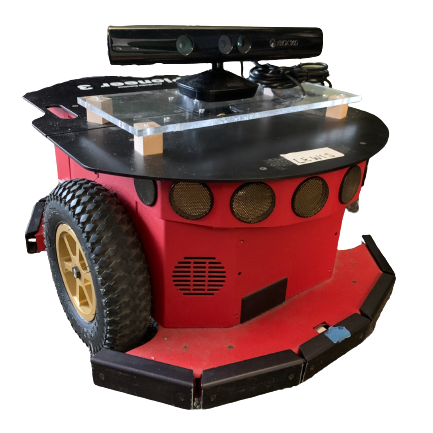
\includegraphics[width=0.5\tikzwidth]{assets/hardware.png}
          };
          \node[block][right=1ex of hardware, yshift=0.165\tikzwidth](kinect) {
            \textbf{Microsoft Kinect}\\\vspace{1ex}
            \small
            \begin{tabular}{l c l}
              RGB Camera&:&640x480, 30fps\\
              IR Camera&:&320x240, 30fps\\
              Max Depth&:&4m\\
            \end{tabular}
          };
          \node[block][below=1ex of kinect](pioneer) {
            \textbf{Pioneer 3-DX}\\\vspace{0.5ex}
            \small
            \begin{itemize}
              \setlength{\itemindent}{-3.5ex}
              \setlength{\itemsep}{-0.55ex}
              \item Two wheel differential drive
              \item Wheel encoders for odometry
              \item 8 front + 8 rear sonar sensors
              \item ROS compatible (using p2os)
              \item Supports velocity control
              \item 8-10 hours of runtime
            \end{itemize}
          };
          \node[block, text width=\tikzwidth-0.3ex, xshift=0.254\tikzwidth][below=1ex of hardware](laptop) {
            \textbf{Compute Unit}\\\vspace{0.3ex}
            \small
            Laptop running Robot Operating System (ROS) on linux (Ubuntu).\\
            Pentium N4200 | 8GB DDR3 RAM | 240 GB SSD
          };

          \draw[draw=orange, ultra thick] (kinect) -- (0,3.5);
          \draw[fill=orange!20] (0,3.5) circle (6pt);
          \draw[draw=orange, ultra thick] (0,3.5) circle (8pt);
          \draw[draw=orange, ultra thick] (pioneer) -- (1.5,-1);
          \draw[fill=orange!20] (1.5,-1) circle (6pt);
          \draw[draw=orange, ultra thick] (1.5,-1) circle (8pt);

        \end{tikzpicture}
      }
    \column{.25}
      \block{System Overview}{
        \setlength{\tikzwidth}{\linewidth-10mm}
        \begin{tikzpicture}[
          block/.style={
            rounded corners=0.4ex, font=\normalsize, fill=red!20,text centered,
            text width=0.33\tikzwidth-1ex, anchor=north, inner sep=1ex
          },
          hardware/.style={block, fill=red!20},
          rosnode/.style={block, fill=blue!20},
          rtabmap/.style={block, fill=blue!30},
          roscore/.style={
            font=\large, fill=orange!20, circle,
            text width=0.10\tikzwidth, text centered
          }
        ]
          \node[roscore](roscore) {
            \textbf{ROS}
          };

          \node[rosnode][left=(0.1\tikzwidth) of roscore](freenect) {
            \textbf{Freenect}\\
            Interfaces with the Kinect camera and publishes RGB and depth images.
          };
          \node[hardware][above=0.75em of freenect](kinect) {
            \textbf{Kinect Camera}\\
          };

          \node[rosnode][right=(0.1\tikzwidth) of roscore](p2os) {
            \textbf{P2OS}\\
            Interfaces with the robot chassis and publishes robot odometry data.
          };
          \node[hardware][above=0.75em of p2os](robot) {
            \textbf{Robot Chassis}\\
          };
          
          \node[rosnode, text width=\tikzwidth][below=2.75em of roscore](rtabmap) {
            \textbf{RTAB-Map}\\
            \vspace{1ex}
            \newlength{\innerwidth}
            \setlength{\innerwidth}{\tikzwidth-2ex}
            \begin{tikzpicture}
              \node[rtabmap, text width=(0.5\innerwidth-1.5ex)]
              (mapping) {
                \textbf{Mapping}\\\vspace{0.5ex}
                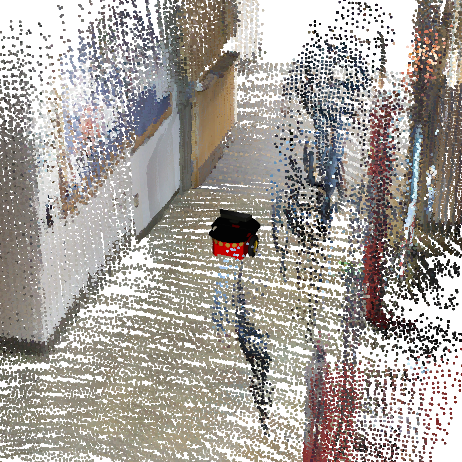
\includegraphics[width=\linewidth]{assets/mapping.png}
                Generates a 3D map of the environment using depht images from 
                the camera and wheel odometry data from the robot. The RGB 
                images are used to extract keypoints for loop closure and 
                landmark recognition.
              };
              \node[rtabmap, text width=(0.5\innerwidth-1.5ex)]
              [right=1ex of mapping](localization) {
                \textbf{Localization}\\\vspace{1ex}
                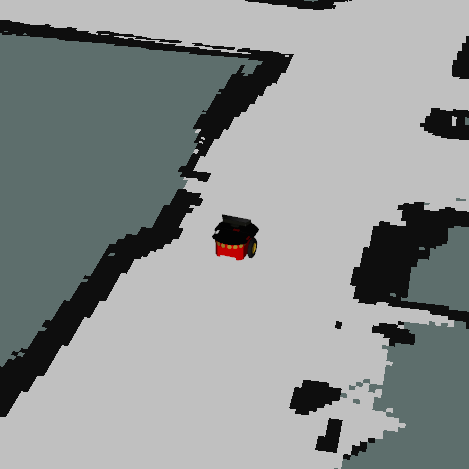
\includegraphics[width=\linewidth]{assets/localization.png}
                Determines the realtime position of the robot in the stored map 
                by extracting keypoints from RGB images and matching them 
                against the landmarks stored in the long term database updated 
                during the mapping process. 
              };
              \node[rtabmap, text width=(\innerwidth), align=justify]
              [below=1ex of mapping, xshift=0.25\innerwidth+0.75ex](memory) {
                \centering\textbf{Long-Term Memeory}\par
                Stores local and global grid maps generated during the mapping 
                process along with keypoints associated with landmarks.
                This is helpful for maintaining information across multiple mapping and
                localization sessions.
              };
            \end{tikzpicture}
            https://github.com/introlab/rtabmap
          };

          \node[rosnode, text width=\tikzwidth, align=justify][above=5em of roscore](mapalign) {
            \centering\textbf{Floor Plan Localization}\par
            Converts the 2D occupancy grid generated by RTAB-Map into a binary 
            mask and applied computer vision techniques such as morphology and 
            feature based template matching to map the position of the agent 
            onto the real world floor plans of the building.
          };
          
          \draw[-latex, line width=1mm] (kinect) -- (freenect);
          \draw[-latex, line width=1mm] (robot) -- (p2os);
          \draw[-latex, line width=1mm] (freenect) -- (roscore);
          \draw[-latex, line width=1mm] (p2os) -- (roscore);
          \draw[-latex, line width=1mm] (rtabmap) -- (roscore);
          \draw[-latex, line width=1mm] (roscore) -- (rtabmap);
          \draw[-latex, line width=1mm] (roscore) -- (mapalign);
          \draw[-latex, line width=1mm] (mapalign) -- (roscore);

        \end{tikzpicture}
      }
    \column{.5}
      \block{Results}{
        
\includegraphics[width=0.3\linewidth]{assets/placeholder.png}\hfill
        
\includegraphics[width=0.3\linewidth]{assets/placeholder.png}\hfill
        
\includegraphics[width=0.3\linewidth]{assets/placeholder.png}\\
        Lorem ipsum dolor sit amet, consectetuer adipiscing elit. Aenean commodo ligula eget dolor. Aenean massa. Cum sociis natoque penatibus et magnis dis parturient montes, nascetur ridiculus mus. Donec quam felis, ultricies nec, pellentesque eu, pretium quis, sem. Nulla consequat massa quis enim. Donec pede justo, fringilla vel, aliquet nec, vulputate eget, arcu. In enim justo, rhoncus ut, imperdiet a, venenatis vitae, justo. Nullam dictum felis eu pede mollis pretium. Integer tincidunt. Cras dapibus. Vivamus elementum semper nisi. Aenean vulputate eleifend tellus. Aenean leo ligula, porttitor eu, consequat vitae, eleifend ac, enim. Aliquam lorem ante, dapibus in, viverra.Lorem ipsum dolor sit amet, consectetuer adipiscing elit. Aenean commodo ligula eget dolor. Aenean massa. Cum sociis natoque penatibus et magnis dis parturient montes, nascetur ridiculus mus. Donec quam felis, ultricies nec, pellentesque eu, pretium quis, sem. Nulla consequat massa quis enim. Donec pede justo, fringilla vel, aliquet nec, vulputate eget, arcu. In enim justo, rhoncus ut, imperdiet a, venenatis
      }
      \begin{subcolumns}
        \subcolumn{.5}
          \block{Conclusion}{
            
          }
        \subcolumn{.5}
          \block{Future Work}{
            
          }
      \end{subcolumns}
  \end{columns}

  \nocite{*}
  \node [anchor=south west, text width=\textwidth,
  fill=titlebgcolor, text=titlefgcolor]at (bottomleft) {
    \begin{tikzpicture}
      \node [text width=0.94\linewidth-1.5em](references) {
        \renewcommand*{\bibfont}{\normalfont\small}
        \color{titlefgcolor}
        \printbibliography[heading=none]
      };
      \node [text width=0.06\linewidth][right=1em of references](qr) {
        
\includegraphics[width=0.75\linewidth]{assets/qr-code.png}
      };
    \end{tikzpicture}
  };
\end{document}